\chapter[Ranking Computer Vision Service Issues using Emotion]
{Ranking Computer Vision Service Issues using Emotion\pubfootnote{Cummaudo:2021semotion}}
\label{ch:semotion2021}
\graphicspath{{mainmatter/publications/figures/semotion2021/}}

% Macros
\def\SEMNumTotalPostsFromSO{1,425}
\def\SEMNumTotalNonNoisePosts{1,239}
\def\SEMNumBeyerClassificationsMade{1,825}
\def\SEMNumClassificationsFromBeyerNonIRRAnalysis{1,375}
\def\SEMNumClassificationsFromBeyerIRRAnalysis{450}
\def\SEMNumNoisyPosts{186}
\def\SEMNumEmoTxtClassifications{1,412}
\def\SEMNumEmotionsDetected{792}
\def\SEMNumNoEmotionsDetected{620}
\def\SEMNumIRRPostsTiedMajority{four}
\def\SEMNumQuestionsOneEmo{1,096}
\def\SEMNumQuestionsTwoEmo{114}
\def\SEMNumQuestionsThreeEmo{28}
\def\SEMNumQuestionsFourEmo{one}
\def\SEMPctNoEmotionAPIUsage{41.46\%}
\def\SEMPctNoEmotionDiscrepancy{43.39\%}
\def\SEMPctNoEmotionErrors{48.36\%}
\def\SEMPctNoEmotionReview{40.77\%}
\def\SEMPctNoEmotionConceptual{43.66\%}
\def\SEMPctNoEmotionAPIChange{31.25\%}
\def\SEMPctNoEmotionAverage{42.10\%}
\def\SEMPctFearAverage{16.77\%}
\def\SEMPctJoyAverage{8.85\%}
\def\SEMPctLoveAverage{8.15\%}
\def\SEMPctSadnessAverage{4.53\%}
\def\SEMPctSurpriseAverage{14.82\%}
\def\SEMPctAngerAverage{4.77\%}

\glsresetall
\begin{abstract}
Software developers are increasingly using \glslongpl{iws} to implement `intelligent' features. However, studies show that incorporating \glslong{ml} into an application increases technical debt, creates data dependencies, and introduces uncertainty due to their non-deterministic behaviour. We know very little about the emotional state of software developers who have to deal with such issues; a reduced developer experience when using such services results in productivity loss. In this paper, we conduct a landscape analysis of emotion found in \SEMNumTotalPostsFromSO{} \glslong{so} questions about \glslongpl{cvs}. We used an existing emotion classifier, EmoTxt, and manually verified its classification results. We found that the emotion profile varies for different types of questions, and a discrepancy exists between automatic and manual emotion analysis due to subjectivity.
\end{abstract}

\glsresetall
\glsunset{api}

\section{Introduction}
Recent advances in \gls{ai} have provided software engineers with new opportunities to incorporate complex \gls{ml} capabilities, such as computer vision, through cloud-based \glspl{iws}. These new set of services, typically offered as \glsac{api} calls are marketed as a way to reduce the complexity involved in integrating \glsac{ai}-components. However, recent work shows that software engineers struggle to use these \glspl{iws}~\citep{Cummaudo:2020icse}. 
Furthermore, the accompanying documentation fails to address common issues experienced by software engineers and often, engineers resort to online communication channels, such as \gls{so}, to seek advice from their peers~\citep{Cummaudo:2020icse}.

While seeking advice on the issues, software engineers tend to express their emotions (such as frustration or confusion) within the questions. Emotions with negative sentiment have been shown to have adverse effects to developer productivity, as shown in \citep{wrobel2013}, and thus---recognising the value of considering emotions---other literature has investigated how emotions are expressed by software developers within communication channels~\citep{ortu2016} including \gls{so}~\citep{novielli2018, calefato2018}. The broad motivation of these works is to generally understand the emotional landscape and improve developer productivity~\citep{murgia2014, ortu2016, gachechiladze2017}. However, previous works have not directly focused on the nature of emotions expressed in questions related to \glspl{iws}. We also do not know if certain types of questions express stronger emotions. Thus, understanding the emotional state of developers facing issues with these services can help shed light into prioritised choices of these services, avoid common issues which are the most frustrating (and thus highest productivity loss), and ultimately improve the developer experience (DevX) whilst using these services.

The machine-learnt behaviour of these cloud \glspl{iws} is typically non-deterministic and, given the dimensions of data used, their internal inference process is hard to reason about~\citep{Cummaudo:2019icsme}. Compounding the issue, documentation of these cloud systems does not explain the limits, nor how they were created (esp. information about the datasets used to train them). This lack of transparency makes it difficult for even senior developers to properly reason about these systems, so their prior experience and anchors do not offer sufficient support~\citep{Cummaudo:2020icse}. In addition, adding machine learned behaviour to a system incurs ongoing maintenance concerns~\citep{Sculley2015}. There is a need to better understand emotions expressed by developers; as reduced negative emotions whilst writing software can improve productivity \citep{wrobel2013} and DevX, we can use such insight to help cloud vendors make improvement which would generate the most value, e.g., overall service/\glsac{api} design, documentation of the services or clarification in error messages.

In our recent work~\citep{Cummaudo:2020icse}, we explored the types of pain-points developers face when using \glspl{iws} through a general analysis of \SEMNumTotalPostsFromSO{} \gls{so} questions using an existing \gls{so} question type classification taxonomy~\citep{Beyer:2018fm} (presented in \cref{semotion2021:tab:taxonomies}). This study extends this body of work by considering the \textit{emotional state} expressed within those same pain-points. We identify the emotion(s) in each \gls{so} question (if any), and investigate if the distribution of these emotions is similar across the various types of questions. To automate classification of these emotions, we used EmoTxt, an emotion classifier included in the EMTk toolkit for emotion recognition from text~\citep{novielli2018, calefato2018, calefato2017}. EmoTxt has been trained and built on \gls{so} posts using the emotion classification model proposed by~\citet{shaver1987}. Additionally, we manually classified a sample of 300 posts using the same guidelines used to train EmoTxt, provided in \citep{novielli2018} (based on \citep{shaver1987}). The key contributions of this study are:

\begin{itemize}
    \item Identifying that the distribution of emotions is different across the taxonomy of issues.
    \item A deeper analysis of the results obtained from the EmoTxt classifier suggests that the classification model needs further refinement. \textit{Love} and \textit{joy}, the least expected emotions when discussing \glsac{api} issues, are visible across all categories.
    \item In order to promote future research and permit replication, we make our dataset publicly available.\footnote{See \url{https://bit.ly/2RIGQ2N}.}
\end{itemize}

The paper is structured as follows: \cref{semotion2021:sec:emotion-mining} provides an overview on prior work surrounding the classification of emotions from text; \cref{semotion2021:sec:methodology} describes our research methodology;  \cref{semotion2021:sec:findings} presents the results from the EmoTxt classifier;  \cref{semotion2021:sec:discussion} provides a discussion of the results obtained; 
\cref{semotion2021:sec:threats} outlines the threats to validity; \cref{semotion2021:sec:conclusion} presents the concluding remarks.  

\section{Motivation}\label{semotion2021:sec:emotion-mining}

Developing software raises various emotions in developers at different times, including enjoyment, frustration, satisfaction, even fear and rage \cite{wrobel2013,ortu2016,wrobel2020,calefato2017}

Studies on the role of emotions within the workplace, including the software engineering domain, have established a correlation between emotion and productivity ~\citep{wrobel2013, wrobel2020}. Negative emotions impact productivity negatively, whilst positive emotions impact positively. The exception is \textit{anger}, which was found to generate a motivating state to ``try harder'' in a subset of developers (i.e., 13\% of respondents in \citeauthor{wrobel2013}'s study \citep{wrobel2013} responded that anger had a \textit{positive} impact to make developers more motivated.  However, overall, \textit{anger} was still found to have an negative impact on productivity). In recent years, researchers have focused on identifying the emotions expressed by software engineers within communication channels such as JIRA to communicate with their peers ~\citep{murgia2014, ortu2016, gachechiladze2017, novielli2018}. Most of these studies make use of one of the well established emotion classification framework during their emotion mining process. ~\citet{murgia2014} and~\citet{ortu2016} investigated the emotions expressed by developers within an issue tracking system, such as JIRA, by labelling issue comments and sentences written by developers using Parrott's emotion framework. ~\citet{gachechiladze2017} applied the Shaver's emotion framework to detect anger expressed in comments written by developers in JIRA. 

The Collab team~\citep{calefato2017, novielli2018} extended the work done by~\citet{ortu2016} and developed an emotion mining toolkit, EmoTxt~\citep{calefato2017} based on a gold standard dataset collected from 4,800 \gls{so} posts (of type questions, question comments, answers and answer comments). 12 graduate computer science students were recruited as raters to manually annotate these 4,800 \gls{so} posts using the Shaver's emotion model which consists of a tree-structured, three level, hierarchical classification of emotions. The top level consists of six basic emotions namely, love, joy, anger, sadness, fear and surprise~\citep{shaver1987}. The work conducted by the Collab team is most relevant to our study since their focus is on identifying emotion from \gls{so} posts and their classifier is trained on a large dataset of \gls{so} posts. Unlike their study, we focus on a single domain (\glslongpl{cvs} or \glsacpl{cvs}) to analysing emotion, as opposed to a wide spectrum of domains. Further, we validate our work with a smaller group of people---diverse in age and cultural backgrounds---to gather a wider sense of emotion classification (i.e., due to the subjective nature of emotions). Lastly, in this work, our intent is to analyse the questions only (not all types of posts) to understand the frustration faced at the time the developers face an issue with the service.

\section{Methodology}\label{semotion2021:sec:methodology}

\subsection{Dataset}

This paper extends our existing work by utilising our previously curated dataset of \SEMNumTotalPostsFromSO{} \gls{so} questions on four popular \gls{cvs} providers: Google Cloud Vision, Amazon Rekognition, Azure Computer Vision, and IBM Watson. Each question is assigned a question type per the taxonomy prescribed in \citet{Beyer:2018fm} (for reference, we provide our interpretation of this taxonomy within \cref{semotion2021:tab:taxonomies}). For further details on how this dataset was produced, we refer to the original paper~\citep{Cummaudo:2020icse}.

After performing additional cleansing of this dataset (to remove noise), we performed \textit{both} automatic and manual emotion classification based on \citeauthor{shaver1987}'s emotion taxonomy \citep{shaver1987}. Automatic emotion detection was performed using using the EmoTxt classifer, and manual classification was performed by three co-authors on a sample of 300 posts. We calculated the inter-rater reliability between EmoTxt and our manually classified questions in two ways: (i)~to see the overall agreement between the three raters in applying the \citeauthor{shaver1987} emotions taxonomy, and (ii)~to see the overall agreement with EmoTxt's classifications. Additional dataset cleansing and results from manual and automatic emotion classification are available online at \url{https://bit.ly/2RIGQ2N}.

\begin{table*}[tb]
    \centering
    \caption[Our interpretations from a Stack Overflow question type taxonomy]{Descriptions of dimensions from our interpretation of \citeauthor{Beyer:2018fm}'s \gls{so} question type taxonomy.}
    \label{semotion2021:tab:taxonomies}
    \small
    \begin{tabular}{p{.2\linewidth}p{.75\linewidth}}
      \toprule
  
      \textbf{Dimension} & \textbf{Our Interpretation}
      \\
      \midrule
      
      \textbf{\glsac{api} usage\dotfill} &
      Issue on how to implement something using a specific component provided by the \glsac{api}
      \\
  
      \textbf{Discrepancy\dotfill} &
      The questioner's \textit{expected behaviour} of the \glsac{api} does not reflect the \glsac{api}'s \textit{actual behaviour}
      \\
  
      \textbf{Errors\dotfill} &
      Issue regarding an error when using the \glsac{api}, and provides an exception and/or stack trace to help understand why it is occurring
      \\
  
      \textbf{Review\dotfill} &
      The questioner is seeking insight from the developer community on what the best practices are using a specific \glsac{api} or decisions they should make given their specific situation
      \\
  
      \textbf{Conceptual\dotfill} &
      The questioner is trying to ascertain limitations of the \glsac{api} and its behaviour and rectify issues in their conceptual understanding on the background of the \glsac{api}'s functionality
      \\
  
      \textbf{\glsac{api} change\dotfill} &
      Issue regarding changes in the \glsac{api} from a previous version
      \\
  
      \textbf{Learning\dotfill} &
      The questioner is seeking for learning resources to self-learn further functionality in the \glsac{api}, and unlike discrepancy, there is no specific problem they are seeking a solution for
      \\
      \bottomrule 
    \end{tabular}
  \end{table*}

\subsection{Additional Dataset Cleansing}
\label{semotion2021:ssec:method:filtering:classification}

As described in \citep{Cummaudo:2020icse}, the \SEMNumTotalPostsFromSO{} questions extracted were split into 5 random samples. The first author classified the first sample of  475 questions, with three other research assistants\footnote{Software engineers in our research group with at least 2 years industry experience} classifying the remaining 900 questions over samples of 300 posts. The remaining 50 posts were used for reliability analysis, whereby these 50 posts were classified nine times by various researchers in our group, resulting in a total of \SEMNumClassificationsFromBeyerIRRAnalysis{} classifications for the 50 posts.

Each question was classified a question issue type (as described by \cref{semotion2021:tab:taxonomies}) or, where the question was a false-positive resulting from our original search query, we flagged the post as `noise' and removed them from further classification. \SEMNumNoisyPosts{} posts were flagged as noise, with a total of \SEMNumTotalNonNoisePosts{} were successfully assigned a question type.

To remove duplicity resulting from the reliability analysis, we applied a `majority rules' technique to each of these 50 posts, in which the issue type most consistent amongst the nine raters per question would win. As an example, three raters classified a post as \textit{\glsac{api} Usage}, one rater classified the same post as a \textit{Review} question and {five} raters classified the post as \textit{Conceptual}. Therefore, the question was assigned as a \textit{Conceptual} question. However, in \SEMNumIRRPostsTiedMajority{} cases, there was a tie in the majority. To resolve this, we used the issue type that was most assigned within the 50 posts. For example, in another question, three raters each assigned the same post as \textit{Discrepancy} and \textit{Errors}, while the remaining three three raters flagged the post as noise. In this case, the tie was resolved down to \textit{Errors} as this classification received 72 more votes than \textit{Discrepancy} and 88 more votes than noisy posts across all classifications made in the sample of 50 posts. 

\subsection{Automatic Emotion Classification}

After all questions had been classified an issue type, we then piped in the body of each question into a script developed to remove all HT\gls{ml} tags, code snippets, blockquotes and hyperlinks, as suggested by~\citet{novielli2018}. We replicated and extended the study conducted by~\citet{novielli2018} on our dataset consisting of questions only.
We started with a file containing the \SEMNumTotalNonNoisePosts{} non-noise \gls{so} questions, each with its associated question type given in \cref{semotion2021:tab:taxonomies}. We pre-processed this file by extracting the question ID and body text to meet the format requirements of the EmoTxt classifier~\citep{calefato2017}. This classifier was used as it was trained on \gls{so} posts as discussed in \cref{semotion2021:sec:emotion-mining}. We ran the classifier for each emotion as this was required by EmoTxt model. This resulted in six output prediction files (one file for each emotion: \textit{Love}, \textit{Joy}, \textit{Surprise}, \textit{Sadness}, \textit{Fear}, \textit{Anger}), which referenced a question ID and a binary value indicating emotion presence. We then merged these emotion prediction files into an aggregate file with question text and~\citeauthor{Beyer:2018fm}'s question type classifications that was performed in \citep{Cummaudo:2020icse}.

\subsection{Manual Emotion Classification} 
\label{semotion2021:ssec:manual}
\def\cohen{$C_{\kappa}$}
\def\light{$L_{\kappa}$}

In order to evaluate and also better understand the process used by EmoTxt to classify emotions, we randomly sampled 300 \gls{so} posts of various emotion annotations resulting from EmoTxt. Each of these 300 posts were assigned to three raters (co-authors of this paper) who individually reviewed the question text against each of the six basic emotions~\citep{shaver1987} and flag an emotion if deemed present, otherwise flagging \textit{No Emotion} instead. Each rater reviewed each question against the guidelines provided in \citep{novielli2018}. We then conducted reliability analysis of all three rater's results to measure the similarity in which independent raters classified each emotions against each \gls{so} post. This was done by calculating Cohen's Kappa (\cohen{})~\citep{Cohen:1960tf} to measure the average inter-rater agreement \textit{between} pairs of raters, and then Light's Kappa (\light{})~\citep{Light:1971vz} to measure the \textit{overall} agreement amongst the three raters. Results are reported in \cref{semotion2021:tab:irr-results}.

\subsection{Comparing Manual and Automatic Classification Methods}

The next step involved comparing the ratings of the 300 \gls{so} posts that were manually annotated by the three raters against the results obtained for the same set of 300 \gls{so} posts from the EmoTxt classifier.
We separated the classifications per emotion and calculated \cohen{} for each rater against EmoTxt, and then \light{} to measure the overall agreement. The three raters then met together to compare and discuss the ratings from the EmoTxt classifier against the manual ratings. Results are reported in \cref{semotion2021:tab:irr-results}.

\section{Findings}\label{semotion2021:sec:findings}

\begin{figure}[t]
\centering
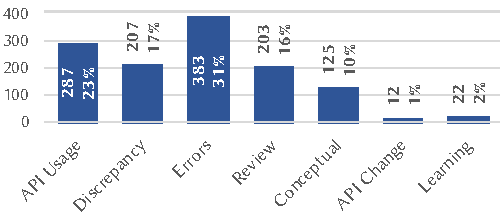
\includegraphics[width=.6\linewidth]{beyerclass}
\caption[Distributions of the types of questions raised]{Distribution of the types of questions raised.}
\label{semotion2021:fig:beyer-classifications}
\end{figure}

\Cref{semotion2021:fig:beyer-classifications} displays the overall distribution of question types from the \SEMNumTotalNonNoisePosts{} posts after applying noise-filtering and majority ruling to our original \SEMNumTotalPostsFromSO{} questions extracted. It is evident that developers ask issues predominantly related to \glsac{api} errors when using \glspl{cvs} and, additionally, how they can use the \glsac{api} to implement specific functionality. There are few questions related to version issues or self-learning. For further discussion into these results, we refer to \citep{Cummaudo:2020icse}.

\begin{table}[th]
\caption{Frequency of emotions per question type.}
\label{semotion2021:tab:emotion-freq}
\tablefit{\begin{tabular}{l|ccccccc|c}
\toprule
\textbf{Question Type}&
\textbf{Fear}&
\textbf{Joy}&
\textbf{Love}&
\textbf{Sadness}&
\textbf{Surprise}&
\textbf{Anger}&
\textbf{No Emotion}&
\textbf{Total}\\
\midrule
\glsac{api} Usage&47&22&34&17&59&13&136&328\\
Discrepancy&35&12&17&7&46&20&105&242\\
Errors&73&34&23&21&47&23&207&428\\
Review&35&16&15&16&42&14&95&233\\
Conceptual&27&9&10&8&21&5&61&141\\
\glsac{api} Change&4&2&2&1&1&1&5&16\\
Learning&3&4&2&0&4&0&11&24\\
\midrule
Total&224&99&103&70&220&76&620&1412\\
\bottomrule
\end{tabular}}
\end{table}

\Cref{semotion2021:tab:emotion-freq} displays the frequency of questions that were classified by EmoTxt when compared to our assignment of question types. \cref{semotion2021:fig:emotion-dist} presents the emotion data proportionally across each type of question. In total, \SEMNumEmotionsDetected{} emotions were detected within the \SEMNumTotalNonNoisePosts{} non-noisy posts, and \SEMNumNoEmotionsDetected{} questions where EmoTxt predicted  \textit{No Emotion} for all the emotion classification runs.
Of the \SEMNumEmotionsDetected{} questions with emotion detected, \SEMNumQuestionsTwoEmo{} questions had two emotions predicted, \SEMNumQuestionsThreeEmo{} questions had three emotions detected, and \SEMNumQuestionsFourEmo{} question\footnote{See \url{http://stackoverflow.com/q/55464541}.} had four emotions detected (\textit{Surprise}, \textit{Sadness}, \textit{Joy} and \textit{Fear}). 

{\textit{No Emotion} was the most prevalent across all question types}, which is consistent with the findings of the Collab group during the training of the EmoTxt classifier. Questions classified as \textit{\glsac{api} Change} had the broadest distribution of emotions, with EmoTxt reporting \SEMPctNoEmotionAPIChange{} of these types of questions as \textit{No Emotion}, compared to overall average of \SEMPctNoEmotionAverage{}. However, this is likely due to the low sample size of \textit{\glsac{api} Change} questions (with only 12 questions assigned this issue type). The next highest set of emotive questions are found in the second and fourth largest samples (\textit{Review} at 203 posts, and \textit{\glsac{api} Usage} at 287 posts); therefore, higher proportions of emotion is not necessarily correlated to sample size.  

Unsurprisingly, \textit{Discrepancy}-based questions---indicative of the frustrations developers face when the \glsac{api} does something unexpected---{had the highest proportion of \textit{Anger} detected}, at 8.26\%, compared to \textit{Anger}'s mean of \SEMPctAngerAverage{}. To our surprise, {\textit{Love} (which we expected least by software developers when encountering issues) was present across all of the different question types}. On average, this was reported at \SEMPctLoveAverage{}. {The two highest emotions, by average, were \textit{Fear} ($\mu=$\SEMPctFearAverage{})and \textit{Surprise} ($\mu=$\SEMPctSurpriseAverage{})}. In contrast, to our surprise, {the two least-detected emotions reported by EmoTxt were \textit{Sadness} ($\mu=$\SEMPctSadnessAverage{}) and \textit{Anger} ($\mu=$\SEMPctAngerAverage{}\%)}. { \textit{Joy} and \textit{Love} were roughly the same}, and fell in between the two proportion ends, with means of \SEMPctJoyAverage{} and \SEMPctLoveAverage{}, respectively.

\begin{table*}[th]
\caption[Inter-rater agreement between human and automatic classifiation]{Inter-rater agreement between humans ($R_{1..3}$) and EmoTxt ($E$) and indicative guidelines of strength.}
\label{semotion2021:tab:irr-results}
\tablefit{\begin{tabular}{l|cccc|cccc}
\toprule
\textbf{Emotion}&
$\mathbf{C_{\kappa}(R_{1},R_{2})}$&
$\mathbf{C_{\kappa}(R_{1},R_{3})}$&
$\mathbf{C_{\kappa}(R_{2},R_{3})}$&
$\mathbf{L_{\kappa}(R_{1..3})}$&
$\mathbf{C_{\kappa}(R_{1},E)}$&
$\mathbf{C_{\kappa}(R_{2},E)}$&
$\mathbf{C_{\kappa}(R_{3},E)}$&
$\mathbf{L_{\kappa}(R_{1..3},E)}$\\
\midrule
Love&0.30~\textit{Fair}&0.17~\textit{Slight}&0.04~\textit{Slight}&\textbf{0.17~\textit{Slight}}&0.37~\textit{Fair}&0.27~\textit{Fair}&0.05~\textit{Slight}&\textbf{0.20~\textit{Slight}}\\
Joy&0.21~\textit{Fair}&0.16~\textit{Slight}&0.57~\textit{Fair}&\textbf{0.31~\textit{Fair}}&0.1~\textit{Slight}&0.07~\textit{Slight}&-0.01~\textit{Poor}&\textbf{0.18~\textit{Slight}}\\
Surprise&0.21~\textit{Fair}&0.13~\textit{Slight}&0.15~\textit{Slight}&\textbf{0.16~\textit{Slight}}&0.17~\textit{Slight}&0.04~\textit{Slight}&0.06~\textit{Slight}&\textbf{0.13~\textit{Slight}}\\
Sadness&0.11~\textit{Slight}&0.05~\textit{Slight}&0.01~\textit{Slight}&\textbf{0.05~\textit{Slight}}&0.09~\textit{Slight}&0.04~\textit{Slight}&0.02~\textit{Slight}&\textbf{0.05~\textit{Slight}}\\
Fear&0.19~\textit{Slight}&0.22~\textit{Fair}&0.36~\textit{Fair}&\textbf{0.26~\textit{Fair}}&-0.02~\textit{Poor}&-0.06~\textit{Poor}&0.01~\textit{Slight}&\textbf{0.12~\textit{Slight}}\\
Anger&0.19~\textit{Slight}&0.19~\textit{Slight}&0.07~\textit{Slight}&\textbf{0.15~\textit{Slight}}&0.13~\textit{Slight}&0.16~\textit{Slight}&0.03~\textit{Slight}&\textbf{0.13~\textit{Slight}}\\
No Emotion&0.30~\textit{Fair}&0.16~\textit{Slight}&0.09~\textit{Slight}&\textbf{0.18~\textit{Slight}}&0.25~\textit{Fair}&0.06~\textit{Slight}&0.04~\textit{Slight}&\textbf{0.15~\textit{Slight}}\\
\bottomrule
\end{tabular}}
\end{table*}

As shown in \cref{semotion2021:tab:irr-results}, results from our reliability analysis between human raters indicated subjectivity in emotion interpretation. Guidelines of indicative strengths of agreement are provided by~\citet{Landis:1977kv}, where $\kappa \leq 0.00$ is \textit{poor} agreement, $0.00 < \kappa \leq 0.20$ is \textit{slight} agreement and $0.20 < \kappa \leq 0.40$ is \textit{fair} agreement. Our assessments across the 300 questions indicate slight agreement for \textit{Love}, \textit{Surprise}, \textit{Sadness}, \textit{Anger} and \textit{No Emotion}, and fair agreement for \textit{Joy} and \textit{Fear}. When combining human raters and EmoTxt, the inter-rater agreement was slight across all emotions.  

\begin{figure}[th]
\centering
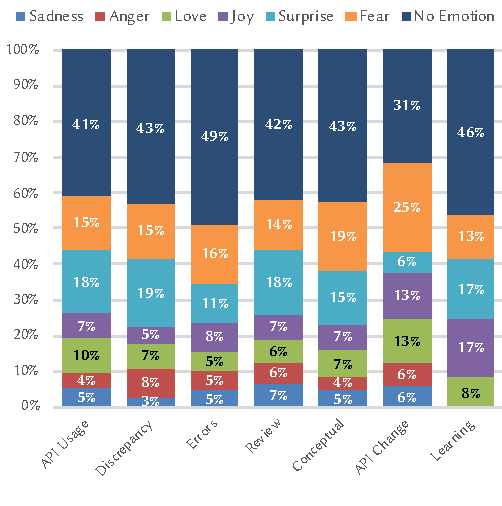
\includegraphics[width=.6\linewidth]{emotionproportion}
\caption[Proportions of emotions per question type]{Proportion of emotions per question type.}
\label{semotion2021:fig:emotion-dist}
\end{figure}

\afterpage{\begin{landscape}
\begin{table*}
\centering
\caption[Sample Stack Overflow questions with emotions identified]{Sample of various question types ([$Q$]) against emotion(s) identified by EmoTxt ([$E$]) and the three raters ([$R_{1..3}$]).}
\label{semotion2021:table:SampleQuestions}
\small
\tablefitlandscape{1}{\begin{tabular}{p{1\linewidth}p{0.2\linewidth}}
\toprule
\textbf{Question ID and Quote}&
\textbf{Classifications}\\

\midrule

\textbf{51444352}:~\textit{``I'm pretty sure I set up my IAM role appropriately (I literally attached the ComprehendFullAccess policy to the role) and the Cognito Pool was also setup appropriately (I know this because I'm also using Rekognition and it works with the IAM Role and Cognito ID Pool I created) and yet every time I try to send a request to AWS Comprehend I get the error... Any idea of what I can do in this situation?''}& 
[$Q$]:~Errors\newline
[$E$]:~Joy\newline
[$R_{1}$]:~Surprise\newline
[$R_{2}$]:~Surprise\newline
[$R_{3}$]:~Anger\medskip\\

{\textbf{53117918}:~\textit{``Ok so I have been stuck here for about more than a week now and I know its some dumb mistake. Just can't figure it out. I am working on a project that is available of two platforms, Android \& iOS. Its sort of a facial recognition app... Is there anything I need to change? Is there any additional setup I need to do to make it work?Please let me know. Thanks.''}}&
[$Q$]:~Discrepancy\newline
[$E$]:~Love, Surprise, Anger\newline
[$R_{1}$]:~Sadness, Anger\newline
[$R_{2}$]:~Sadness, Anger\newline
[$R_{3}$]:~Anger\medskip\\

\textbf{52829583}:~\textit{``I was trying to make the google vision OCR regex searchable... it fails when there is the text of other languages.It's happening because I have only English characters in google vision word component as follows.As I can't include characters from all the languages, I am thinking to include the inverse of above... So where can I find ALL THE SPECIAL CHARACTERS WHICH ARE IDENTIFIED AS A SEPARATE WORD BY GOOGLE VISION? Trial and error, keep adding the special characters I find is one option. But that would be my last option.''}&
[$Q$]:~Review\newline
[$E$]:~Anger\newline
[$R_{1}$]:~Joy, Anger\newline
[$R_{2}$]:~Anger\newline
[$R_{3}$]:~Surprise\medskip\\

\textbf{50190527}:~\textit{``I am trying to perform OCR on pdf documents using google cloud vision \glsac{api}, i uploaded a pdf document into a cloud bucket and downloaded the oauth key file and added it in the script as below. But when i run the file, i get the permission denined: 403 error, can anyone please give me instructions on how to fix it, i did extensive google search and did not yield any results, i am surely missing something here... I have checked the older stack overflow questions and the links provided in answers are not active anymore.Thanks in advance for your help.''}&
[$Q$]:~\glsac{api} Usage\newline
[$E$]:~No Emotion\newline
[$R_{1}$]:~Sadness\newline
[$R_{2}$]:~No Emotion\newline
[$R_{3}$]:~Anger\medskip\\

\textbf{52126752}:~\textit{``I am trying to call google cloud vision api from xamarin C\# android application code.I have set environment variable but still I was not able to call api.So I decided to call it by passing credential json file but now I am getting error deserializing JSON credential datahere is my code''}&
[$Q$]:~Errors\newline
[$E$]:~Surprise\newline
[$R_{1}$]:~No Emotion\newline
[$R_{2}$]:~No Emotion\newline
[$R_{3}$]:~Anger\medskip\\

{\textbf{48145425}:~\textit{``I am Deploying Google cloud vision Ocr in My angular2 webapp. but i am getting many of the errors when i add this code in my webapp code. please help me to sort out this.''}}&
[$Q$]:~Errors\newline
[$E$]:~Fear\newline
[$R_{1}$]:~Fear\newline
[$R_{2}$]:~No Emotion\newline
[$R_{3}$]:~Sadness\\


\bottomrule
\end{tabular}}
\end{table*}\end{landscape}}

\section{Discussion}\label{semotion2021:sec:discussion}

Our findings from the comparison between the manually annotated \gls{so} posts and the automatic classification revealed substantial discrepancies. \Cref{semotion2021:table:SampleQuestions} provides some sample questions\footnote{Questions located at https://stackoverflow.com/q/[ID].} from our dataset, with the \citeauthor{Beyer:2018fm} question classification type noted with [$Q$], the emotion(s) identified by EmoTxt within the text noted with [$E$], and the emotion(s) classified by the three raters indicated with [$R_{1..3}$]. The subset of questions analysed by our three raters do not indicate the automatic (EmoTxt) emotion, and upon manual inspection of the text after poor results from our reliability analysis, an introspection of the dataset sheds some light to the discrepancy. 

For example, the first question in \cref{semotion2021:table:SampleQuestions} shows no indication of \textit{Joy}, but EmoTxt classifies it to this emotion. Phrases like \textit{``I'm \textbf{pretty} sure...''} could be the reason why poor classification occurred, where words like ``pretty'' are associated with \textit{Joy}, albeit in completely different context. It seems likely that the developer is experiencing a confusing situation when the \glsac{api} throws unexpected errors; thus [$R_{1}$] and [$R_{2}$] noting \textit{Surprise}.  Similarly, in the second question presented in \cref{semotion2021:table:SampleQuestions}, EmoTxt classifies \textit{Love}, \textit{Surprise}, and \textit{Anger}. It is difficult to find an element of love or appreciation elsewhere in this context beyond the closing remarks: \textit{``\textbf{Please} let me know. \textbf{Thanks}.''}. Moreover, the disparity between EmoTxt and the agreed emotions between the first two reviewers shows that EmoTxt cannot detect the frustration (\textit{Anger}) in the developer's tone, which is evident in their opening sentence, \textit{``I have been \textbf{stuck here} for about more than a week and I know it is some \textbf{dumb mistake}.''}. 

These results indicate that introspection into the behaviour and limitations of the EmoTxt model is necessary. Our results indicate further work is needed to refine the \gls{ml} classifiers that mine emotions in the \gls{so} context. The question that arises is whether the classification model is truly reflective of real-world emotions expressed by software developers. As highlighted by~\citet{curumsing2017}, the divergence of opinions with regards to the emotion classification model proposed by theorists raises doubts to the foundations of basic emotions. Most of the studies conducted in the area of emotion mining from text is based on an existing general purpose emotion framework from psychology~\citep{Ondrej:2016, ortu2016, novielli2018}---none of which are finely tuned for the software engineering domain. 

\section{Threats to Validity}\label{semotion2021:sec:threats}

\subsection{Internal validity} 
The \textit{\glsac{api} Change} and \textit{Learning} question types were few in sample size (only 12 and 22 questions, respectively). The emotion  proportion distribution of these question types are  quite different to the others.  Given the low number of questions, the sample is too small to make confident assessments. Furthermore, our assignment of~\citeauthor{Beyer:2018fm}'s question type taxonomy was single-label; a multi-labelled approach may work better, however analysis of results would become more complex. A multi-labelled approach would be indicative for future work. 

\subsection{External validity}
EmoTxt was trained on questions, answers and comments, however our dataset contained questions only. It is likely that our results may differ if we included other discussion items, however we wished to understand the emotion within developers' \textit{questions} and classify the question based on the question classification framework by~\citet{Beyer:2018fm}. Moreover, this study has only assessed frustrations within the context of a concrete domain; intelligent \glspl{cvs}. The generalisability of this study to other \glspl{iws}, such as natural language processing services, or conventional web services, may be different. Furthermore, we only assessed four popular \glspl{cvs}; expanding the dataset to include more services, including non-English ones, would be insightful. We leave this to future work.

\subsection{Construct validity}
Some posts extracted from \gls{so} were false positives. Whilst flagged for removal, we cannot guarantee that all false positives were removed. Furthermore, \gls{so} is known to have questions that are either poorly worded or poorly detailed, and developers sometimes ask questions without doing any preliminary investigation. This often results in down-voted questions. We did not remove such questions from our dataset, which may influence the measurement of our results.

\section{Conclusion}\label{semotion2021:sec:conclusion}

We wanted to see how developers emotions are indicated in Stack Overflow (\gls{so}) posts when using \glspl{cvs}. We analysed \SEMNumTotalPostsFromSO{} \gls{so} posts about \glspl{cvs} for emotions using an automated tool and then cross-checked our results manually. We found that the distribution of emotion differs across the taxonomy of issues, and that the current emotion model typically used in recent works is not appropriate for emotions expressed within \gls{so} questions. Consistent with prior work~\citep{lin2018sentiment}, our results demonstrate that \gls{ml} classifiers for emotion are insufficient; human assessment is required.
